% CS 418: Intro to Data Science — Worksheet 25 (25-week13-day1)
% Week 13, Monday 2026-11-16
% NOTICE: This worksheet was drafted by an LLM coding system from the
% instructor's choice of checkpoints. It is maintained, reviewed, and vetted by humans.
% Compile with: latexmk -pdf worksheet.tex

\documentclass[11pt]{article}

% ── Packages ──────────────────────────────────────────────────────────────────
\usepackage[margin=0.65in, headheight=14pt]{geometry}
\usepackage{amsmath, amssymb}
\usepackage{ragged2e}
% Never break a word across lines, including at hyphens ("Sans-Serif").
\hyphenpenalty=10000
\exhyphenpenalty=10000
\usepackage{enumitem}
\usepackage{booktabs}
\usepackage{graphicx}
\usepackage{hyperref}
\usepackage{xcolor}
\usepackage{fancyhdr}
\usepackage{mdframed}
\usepackage{array}

% ── Draft watermark ───────────────────────────────────────────────────────────
% This worksheet is still a draft. The watermark marks the PDF as unfinished so
% nobody mistakes a placeholder for the real thing. Delete this block once the
% worksheet has been reviewed.
\usepackage{draftwatermark}
\SetWatermarkText{IN-PROGRESS}
\SetWatermarkScale{2.2}
\SetWatermarkLightness{0.85}

% ── Page style ────────────────────────────────────────────────────────────────
\pagestyle{fancy}
\fancyhf{}
\lhead{\textbf{CS 418: Intro to Data Science}}
\rhead{UIC, Fall 2026}
\cfoot{\thepage}
\renewcommand{\headrulewidth}{1pt}
\setlength{\headheight}{12pt}
\setlength{\headsep}{0.4cm}

% ── Hyperlinks ────────────────────────────────────────────────────────────────
\hypersetup{colorlinks=false, hidelinks}

% ── Convenience environments ──────────────────────────────────────────────────
% Usage: \blankspace{6cm} — blank area for hand-written work, no rules
\newcommand{\blankspace}[1]{%
  \vspace{0.3em}
  \begin{minipage}[t][#1][t]{\linewidth}
  \end{minipage}
  \vspace{0.3em}
}

% Usage: \guidedopen{title}{guided content}{guided workspace height}{open-ended workspace height}
% Left: a titled prompt with its own blank workspace. Right: a blank workspace for open-ended notes on the same part of the talk, sized so the two columns land at roughly the same height.
\newcommand{\guidedopen}[4]{%
  \noindent\textbf{#1}\\[0.18em]
  \noindent
  \begin{minipage}[t]{0.485\textwidth}
    #2
    \blankspace{#3}
  \end{minipage}
  \hfill
  \begin{minipage}[t]{0.485\textwidth}
    \blankspace{#4}
  \end{minipage}
  \\[0.4em]
}

% ══════════════════════════════════════════════════════════════════════════════
\begin{document}
\RaggedRight

% ── Title block: topic left, info box right ───────────────────────────────────
\noindent
\begin{minipage}[t]{0.55\textwidth}
  \vspace{0pt}
  {\LARGE \textbf{Worksheet \#\,25}} \\[0.18em]
  {\large \textit{Week 13, Day 1: Guest lecture, Ward Wise}} \\[0.18em]
  {\small Sean MacMullan, Chi Hack Night}
\end{minipage}
\hfill
\begin{minipage}[t]{0.40\textwidth}
  \vspace{0pt}
  \small
  Name: \underline{\hspace{4.5cm}} \\[0.35em]
  NetID: \underline{\hspace{4.3cm}} \\[0.35em]
  Date: \underline{\hspace{4.4cm}} \\
\end{minipage}

\vspace{0.6em}
\noindent\rule{\linewidth}{0.6pt}
\vspace{0.1em}

\noindent\underline{\textbf{Guided checkpoints}}\\[0.2em]
\noindent{\small For full credit, fill in the checkpoints. If you skip a checkpoint, you must include your own notes for full credit.}
\vspace{0.8em}

% ── 1. The question ──────────────────────────────────────────────────────────
\guidedopen{1. The Question}{
What question is Ward Wise trying to answer? Write it as one sentence.
}{2.0cm}{3.0cm}

\vfill

% ── 2. Who decides? ──────────────────────────────────────────────────────────
\guidedopen{2. Who Decides?}{
Who decides which cracks and potholes get filled? Write down the people or offices involved, and how the decision gets made.
}{3.2cm}{4.6cm}

\vfill

% ── 3. The data ──────────────────────────────────────────────────────────────
\guidedopen{3. The Data}{
What data does Ward Wise use?

\vspace{0.5em}
Where it comes from:
\vspace{1.2cm}

One row represents:
\vspace{1.2cm}

One problem with it:
}{1.2cm}{5.2cm}

\vfill

\newpage

% ── 4. The lifecycle ─────────────────────────────────────────────────────────
% ds-lifecycle.pdf is docs/assets/lifecycle/ds-lifecycle-v0.svg (the figure in the Week 1, 2, and 10 decks) converted with `rsvg-convert -f pdf`. It spans both columns so its labels stay legible.
\noindent\textbf{4. The Data Science Lifecycle}\\[0.18em]
\noindent Pick one step of the data science lifecycle from Week 1. How did it show up in Ward Wise?

\begin{center}
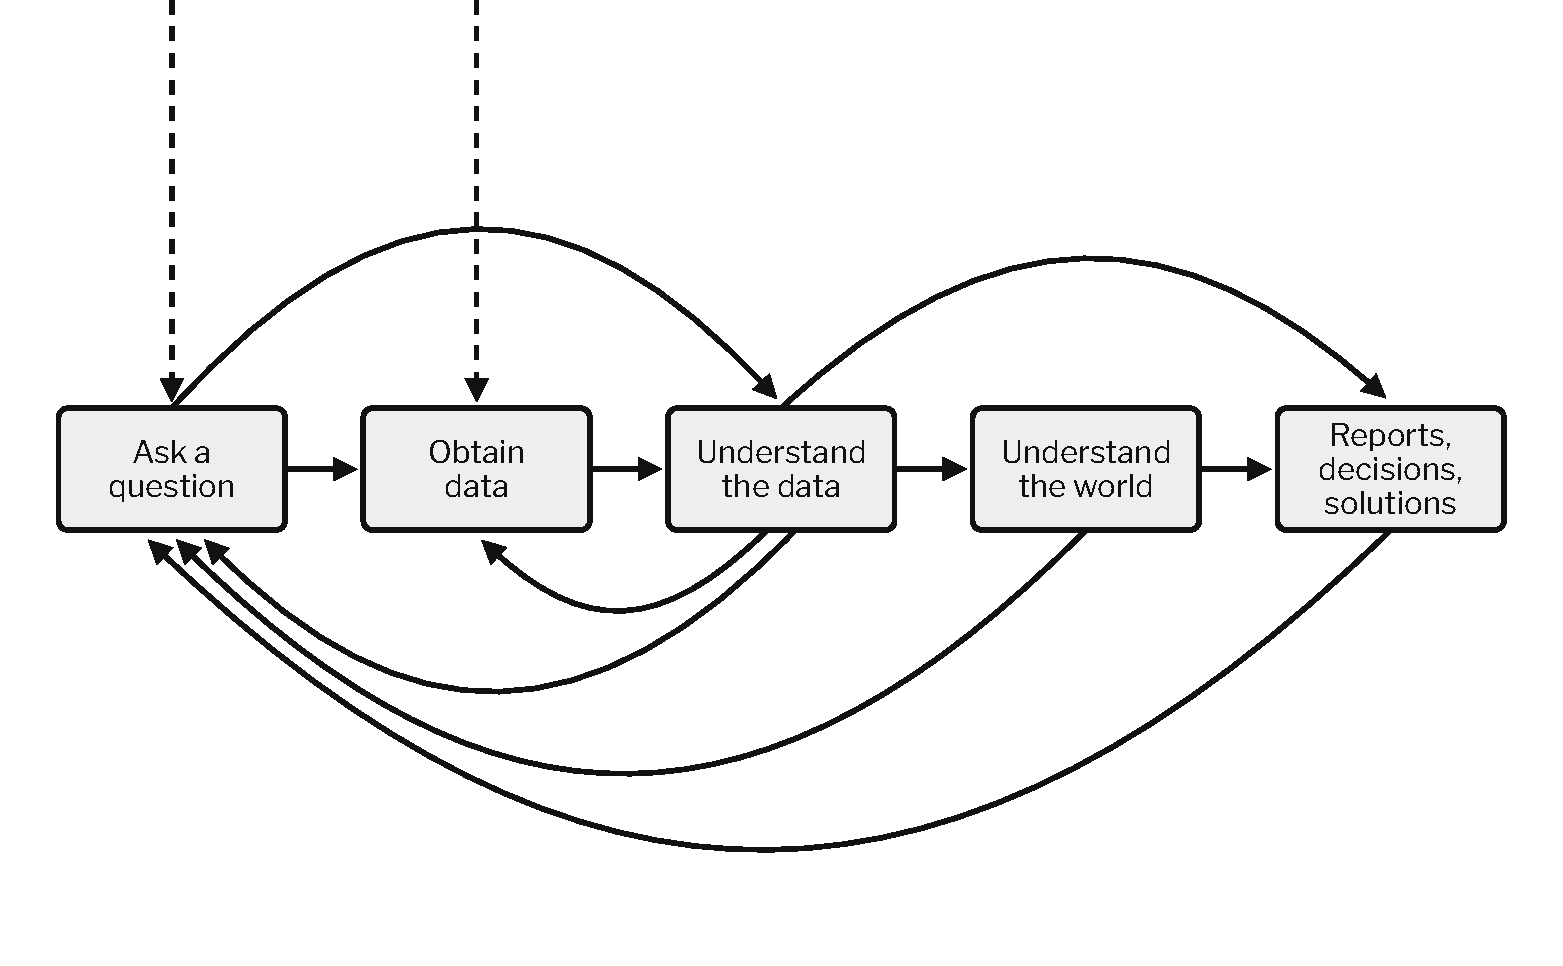
\includegraphics[width=0.75\textwidth]{ds-lifecycle.pdf}
\end{center}

\noindent
\begin{minipage}[t]{0.485\textwidth}
  Step: \underline{\hspace{4.0cm}}
  \blankspace{2.6cm}
\end{minipage}
\hfill
\begin{minipage}[t]{0.485\textwidth}
  \blankspace{3.2cm}
\end{minipage}
\\[0.4em]

\vfill

% ── 5. Your neighborhood ─────────────────────────────────────────────────────
\guidedopen{5. Your Neighborhood}{
Write one question about your own neighborhood that you could ask with this data.
}{2.0cm}{3.0cm}

\vfill

% ── 6. A question for Sean ───────────────────────────────────────────────────
\guidedopen{6. A Question for Sean}{
Write one question you asked, or would like to ask, Sean.
}{1.6cm}{2.6cm}

\vfill

\end{document}
